\begin{figure*}[h!]
    \centering
    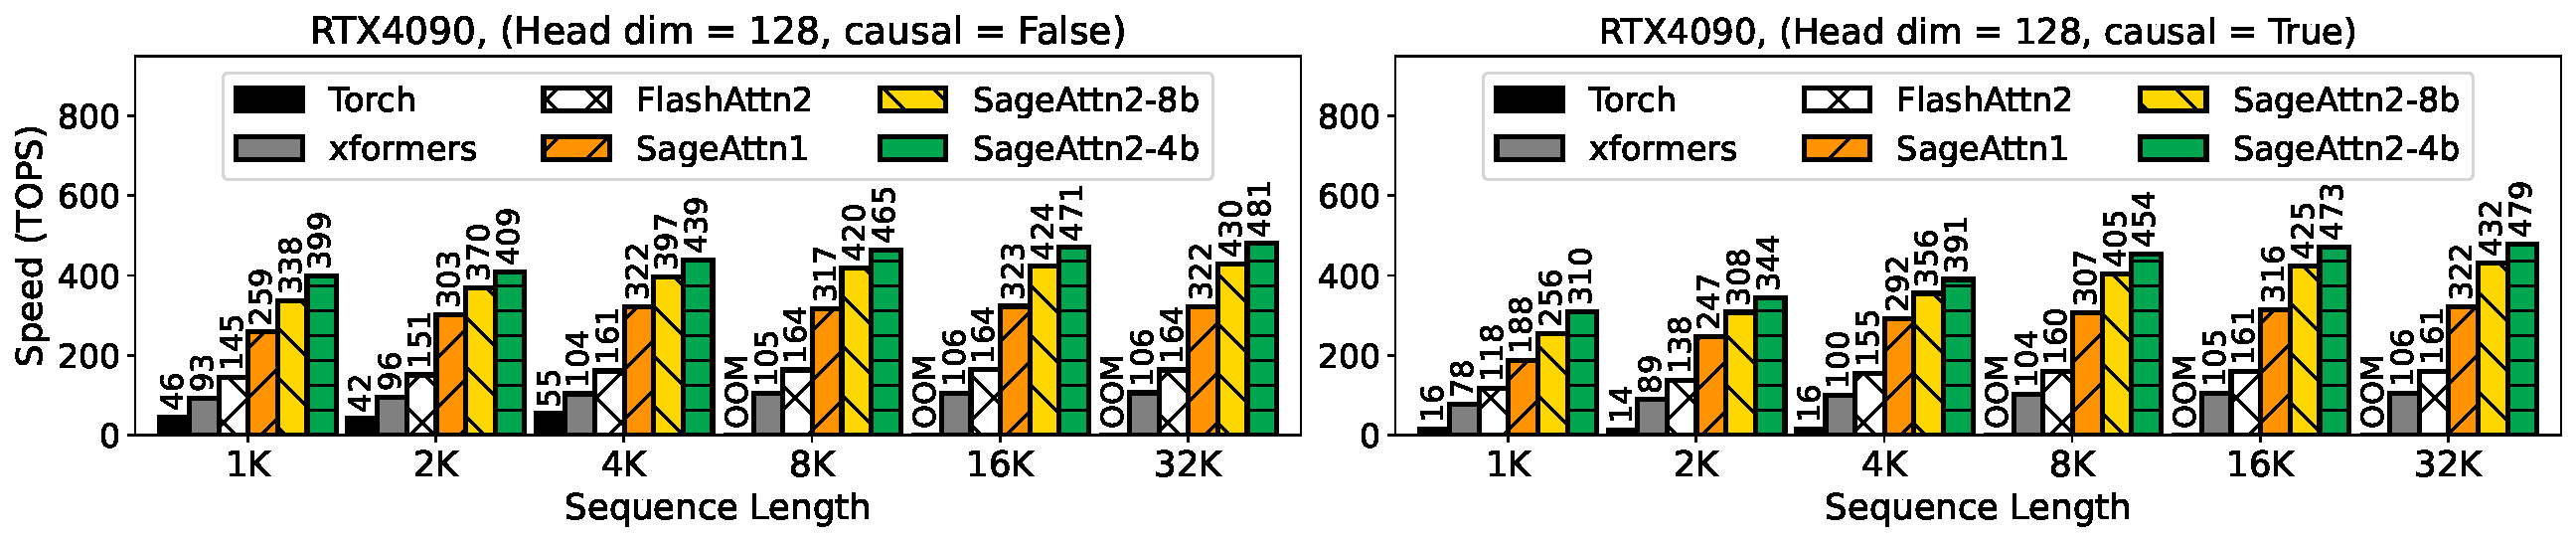
\includegraphics[width=0.97\textwidth]{src/figs/sage_attn2_hd128_baselines_kernel_flops.pdf}
    \vspace{-1.5em}
    \caption{Speed comparison between \our and baselines (RTX4090, headdim=128).}
    \vspace{-1em}
    \label{fig:kf_h128_baseline_RTX4090}
\end{figure*}


\begin{table*}[!t]
\vspace{-.25em}
    \caption{End-to-end metrics across text, image, and video generation models. \ding{55} indicates an inability to generate results for evaluation.}
    \vspace{-.3em}
    \label{exp:metrics_loss_t2t}
    \setlength\tabcolsep{8.1pt}
    \begin{center}
    \scalebox{0.88}{\begin{tabular}{p{2.12cm}|p{3cm}|c|c|c|c}
    \toprule
    {\bf Model}  & {\bf Attention}  & {\bf WikiText (Ppl.) $\downarrow$}  & {\bf Lambda (Acc.) $\uparrow$}  & {\bf MMLU (Acc.) $\uparrow$}  &  {\bf Longbench $\uparrow$}  \\ \hline

    \multirow{6}{*}{\llamal} & Full-Precision & 6.013  & 0.815  & 0.635 & 49.40   \\  
    & \texttt{HadmdAttn} & 7.872 & 0.762  &  0.500  &  44.07  \\
    & \texttt{SmoothAttn} & 7.180 & 0.783  &  0.541  & 44.69   \\
    & \texttt{SageAttention} & \textbf{6.017} &  \textbf{0.812}  & \textbf{0.634}  & \textbf{49.55}  \\
    & \ourf & \textbf{6.256} &  \textbf{0.798}  &  \textbf{0.607}  & \textbf{48.79}  \\ 
    & \oure & \textbf{6.019} &  \textbf{0.811}  &  \textbf{0.634}  & \textbf{49.59} \\ 
      \hline

    \multirow{6}{*}{\glm} & Full-Precision & 7.241 & 0.432  & 0.743 & 49.78   \\  
    & \texttt{HadmdAttn}  & 7.989 &  0.435 &  0.669  &  45.97  \\
    & \texttt{SmoothAttn}  & 8.943 & 0.449  &  0.592  &   42.20 \\
    & \texttt{SageAttention} & \textbf{7.243} &  \textbf{0.433}  & \textbf{0.744}  & \textbf{49.79}  \\
    & \ourf & \textbf{7.352} &  \textbf{0.433}  &  \textbf{0.725}  & \textbf{49.23}  \\ 
    & \oure & \textbf{7.242} &  \textbf{0.432}  &  \textbf{0.745}  & \textbf{49.60}   \\ 
      \bottomrule
    \end{tabular} }
    \end{center}
\vspace*{-.9em}
    \begin{center}
    \setlength\tabcolsep{13.1pt}
    \scalebox{0.88}{\begin{tabular}{p{1.7cm}|p{2.7cm}|c|c|c|c|c}
    \toprule
    {\bf Model}  & {\bf Attention}  & {\bf CLIPSIM $\uparrow$}  & {\bf CLIP-T $\uparrow$}  & {\bf VQA-a $\uparrow$}  & {\bf VQA-t $\uparrow$}  & {\bf FScore $\uparrow$} \\ \hline

    \multirow{6}{*}{\hspace{-.75em}\makecell[c]{\cogvideo\\(1.5-5B)}} & \hspace{-.3em}Full-Precision  & 0.1778 & 0.9979  & 70.231  &  70.928  &  2.507 \\ 
    & \hspace{-.3em}\texttt{HadmdAttn} & 0.1576 &  0.9933 & 8.990  & 2.299   &  \ding{55}  \\
    & \hspace{-.3em}\texttt{SmoothAttn} & 0.1559 & 0.9950  & 8.812  &  2.277  &  \ding{55}   \\
    & \hspace{-.3em}\texttt{SageAttention}  & \ding{55} &  \ding{55}  &  \ding{55}  & \ding{55}  & \ding{55} \\
    & \mbox{\hspace{-.3em}\texttt{FlashAttn3-fp8}}  & 0.1562 & 0.9918 & 6.531 & 2.181 & \ding{55} \\
    & \hspace{-.3em}\ourf  & \textbf{0.1721} &  \textbf{0.9978}  &  \textbf{57.729}  &  \textbf{52.989} & \textbf{2.884} \\ 
    & \hspace{-.3em}\oure  & \textbf{0.1775} &  \textbf{0.9980}  &  \textbf{69.492}  &  \textbf{74.415}  & \textbf{2.487}  \\
     \hline

    \multirow{6}{*}{\hspace{-.5em}\makecell[c]{\texttt{Hunyuan}\\ \texttt{Video}}} & \hspace{-.3em}Full-Precision & 0.1783 & 0.9995  &  82.516 &  75.934  & 0.604    \\  
    & \hspace{-.3em}\texttt{HadmdAttn} & 0.1727 & 0.9989 & 7.514  & 0.762  & 0.175  \\
    & \hspace{-.3em}\texttt{SmoothAttn} & 0.1739 & 0.9988 & 6.987  &  0.609  &  0.148  \\
    & \hspace{-.3em}\texttt{SageAttention}  & \textbf{0.1786} &  \textbf{0.9995}  &  \textbf{82.496}  &  \textbf{79.843}  & \textbf{0.597} \\
    & \mbox{\hspace{-.3em}\texttt{FlashAttn3-fp8}}  & 0.1742 & 0.9941 & 4.433 & 1.460 & \ding{55} \\
    & \hspace{-.3em}\ourf & \textbf{0.1751} &  \textbf{0.9995}  &  \textbf{81.478}  & \textbf{65.371}  &  \textbf{0.610}  \\ 
    & \hspace{-.3em}\oure & \textbf{0.1782} &  \textbf{0.9996}  &  \textbf{81.786}  & \textbf{75.354}  &  \textbf{0.586}  \\
     \hline

    \multirow{6}{*}{\hspace{-.0em}\mochi} & \hspace{-.3em}Full-Precision & 0.1798 &  0.9986 &  45.549 & 65.416   &  1.266  \\  
    & \hspace{-.3em}\texttt{HadmdAttn} & 0.1733 & 0.9980  & 9.053  &  25.133  & 0.704  \\
    & \hspace{-.3em}\texttt{SmoothAttn} & 0.1687 &  0.9978 & 3.383  &  3.480  &  0.241  \\
    & \hspace{-.3em}\texttt{SageAttention}  & \textbf{0.1800} &  \textbf{0.9987}  &  \textbf{48.707}  &  \textbf{63.763}  & \textbf{1.269} \\
    & \mbox{\hspace{-.3em}\texttt{FlashAttn3-fp8}}  & 0.1762 & 0.9982 & 14.964 & 13.711 & 0.457 \\
    & \hspace{-.3em}\ourf & \textbf{0.1783} &  \textbf{0.9986}  &  \textbf{35.955}  & \textbf{43.735}  &  \textbf{1.137}  \\ 
    & \hspace{-.3em}\oure & \textbf{0.1797} &  \textbf{0.9986}  &  \textbf{46.760}  & \textbf{64.901}  &  \textbf{1.255}  \\ 
    \bottomrule
    \end{tabular} }
    \end{center}

\vspace*{-.9em}

    \begin{center}
    \setlength\tabcolsep{27.7pt}
    \scalebox{0.88}{\begin{tabular}{p{0.6cm}|p{1.878cm}|c|c|c|c}
    \toprule
    {\bf Model}  & {\bf Attention}  & {\bf FID $\downarrow$}  & {\bf sFID $\downarrow$}  & {\bf CLIP $\uparrow$}  & {\bf IR $\uparrow$}
    \\ \hline

    \multirow{6}{*}{\hspace{-1.2em}\flux} & \hspace{-1.5em}Full-Precision & 10.960 &  16.648 & 26.180  & 1.009  \\  
    & \hspace{-1.5em}\texttt{HadmdAttn}  & 11.353 & 18.495  & 26.123  &  0.965    \\
    & \hspace{-1.5em}\texttt{SmoothAttn}  & 11.149 &  19.017 & 26.109  &  0.959     \\
    & \mbox{\hspace{-1.86em}\texttt{SageAttention}}  & \textbf{10.944} &  \textbf{16.641}  &  \textbf{26.171}  & \textbf{1.008}  \\
    & \hspace{-1.86em}\ourf  & \textbf{10.577} &  \textbf{17.497}  &  \textbf{26.141}  & \textbf{0.998}  \\ 
    & \hspace{-1.86em}\oure  & \textbf{10.927} &  \textbf{16.723}  &  \textbf{26.175}  & \textbf{1.009}  \\  
       \hline

    \multirow{6}{*}{\hspace{-2.1em}\texttt{\makecell[c]{Stable-Dif\\fusion3.5}}} & \hspace{-1.5em}Full-Precision  & 14.105 & 15.646  &  25.505 & 0.902    \\  
    & \hspace{-1.5em}\texttt{HadmdAttn}  & 14.259 & 15.909  & 25.513  & 0.886     \\
    & \hspace{-1.5em}\texttt{SmoothAttn}  & 14.161 & 15.649  & 25.510  &  0.887      \\
    & \mbox{\hspace{-1.86em}\texttt{SageAttention}}  & \textbf{14.140} &  \textbf{15.678}  &  \textbf{25.503}  & \textbf{0.902}  \\
    & \hspace{-1.86em}\ourf  & \textbf{14.097} &  \textbf{15.397}  &  \textbf{25.487}  & \textbf{0.895}  \\ 
    & \hspace{-1.86em}\oure  & \textbf{14.106} &  \textbf{15.647}  &  \textbf{25.499}  & \textbf{0.901}  \\ 
\bottomrule
    \end{tabular} }
    \end{center}
\vspace{-2em}
\end{table*}


\begin{figure*}[h!]
    \begin{center}
    \vspace{-.5em}
    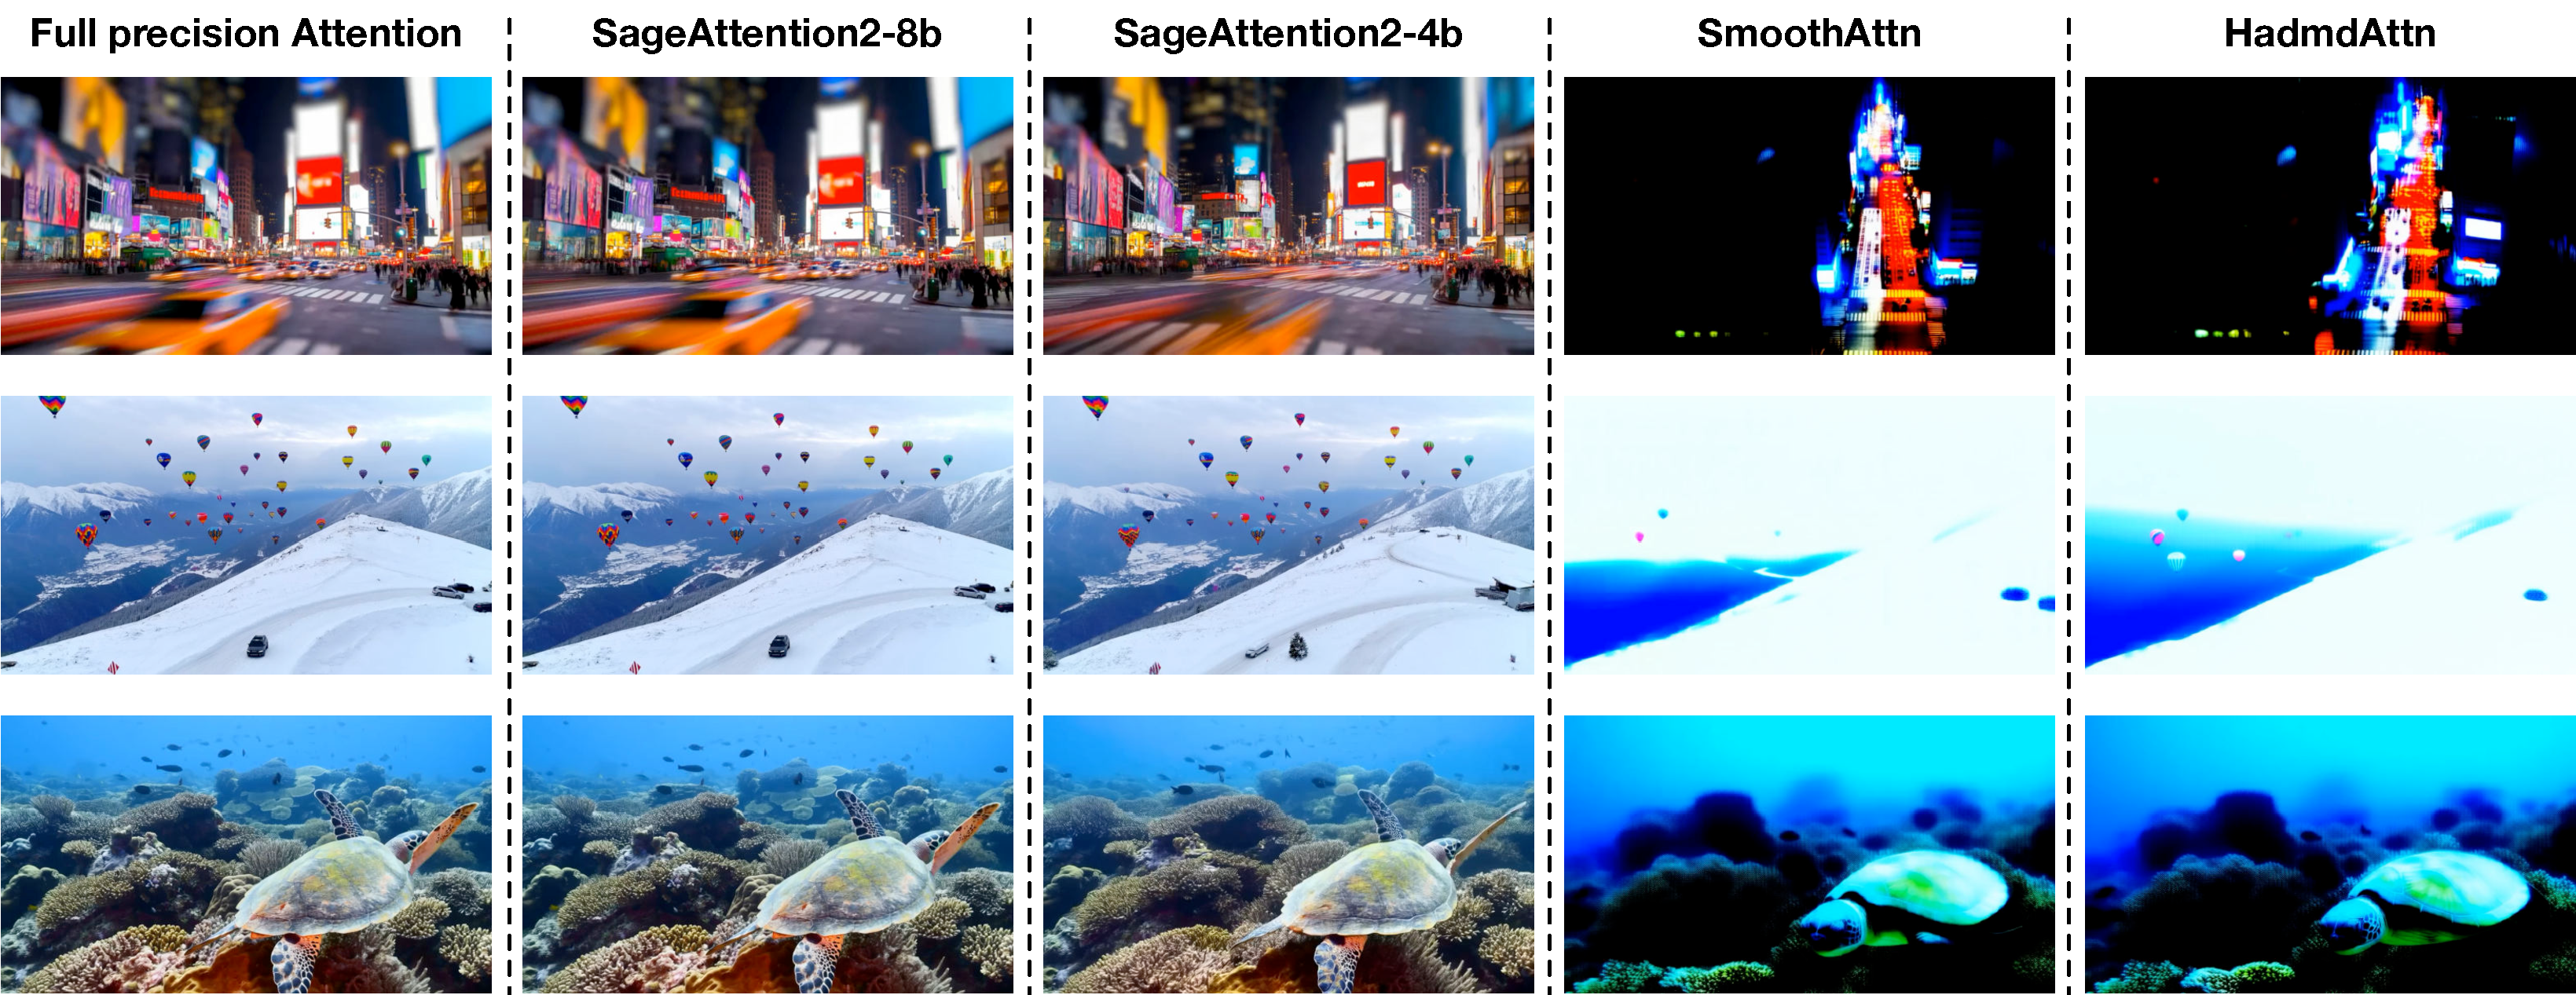
\includegraphics[width=.97\textwidth]{src/figs/comparison_hunyuan.pdf}
    \vspace{-1em}
    \caption{Comparison examples from \hyvideo, prompts are sampled from open-sora prompt sets.}
    \vspace{-.5em}
    \label{fig:hunyuan_example}
    \end{center}
\end{figure*}

\begin{figure*}[h!]
\vspace{-.5em}
    \begin{center}
    \includegraphics[width=1.0\textwidth]{src/figs/FA3_example1.pdf}
    \vspace{-2em}
    \caption{A comparison example using SageAttn2-8b and FlashAttention3 on \cogvideo-1.5.}
    \vspace{-1em}
    \label{fig:video_example1}
    \end{center}
\end{figure*}



\vspace*{-.3em}
\section{Experiment}
\vspace*{-.15em}
\label{sec:exp}
\textbf{Main result.} SageAttention2 is faster than FlashAttention2 and xformers by about \textbf{3x} and \textbf{4.5x}. Moreover, \our matches the speed of FlashAttn3(fp8) on the Hopper GPUs and is much more accurate than FlashAttn3(fp8). SageAttention2 maintains end-to-end metrics across language, image, and video generation models. 
% \vspace{-.5em}

\vspace{-.15em}
\subsection{Setup}
\vspace{-.15em}
\noindent \noindent\textbf{Models.} 
We validate the effectiveness of \our across a diverse set of representative models from language, image, and video generation.
Specifically, we conduct experiments on \uline{ten} models: \llama(7B)~\cite{touvron2023llama2}, \llamal(8B)~\cite{llama31model}, and \glm(9B)~\cite{glm2024chatglm} for text2text, \cogvideo(2B), \cogvideo(1.5-5B)~\cite{yang2024cogvideox}, \hyvideo~\cite{kong2024hunyuanvideo}, and \mochi~\cite{genmo2024mochi} for text2video, \flux(schnell)~\cite{flux} and \sd(turbo)~\cite{stable_diffusion_3_5} for text2image, and \timm~\cite{rw2019timm} for image classification. 

\noindent \noindent\textbf{Datasets and metrics.} For Details about the datasets and metrics we used, please refer to Appendix.~\ref{sec:exp_dataset_metrics}.

\begin{table}[h!]
    \centering
    \vspace{-1.25em}
    \caption{Two kernel implementations of \our.}
    \label{tab:implementation}
    \setlength\tabcolsep{2pt}
    \scalebox{0.85}{
    \begin{tabular}{c|c|c}
        \toprule
        \textbf{Kernel} & $\psi_Q(Q)$, $\psi_K(K)$ & $\psi_P(\widetilde P)$, $\psi_V(V)$ \\
        \hline
        \texttt{SageAttn2-4b}  & INT4 per-thread	 & FP8 per-block and per-channel \\
        \texttt{SageAttn2-8b}  & INT8 per-thread	 & FP8 per-block and per-channel	 \\ 
        \bottomrule                  
    \end{tabular}
    }
\vspace{-1em}
\end{table}

\noindent\textbf{Implemetation.} We implement two attention kernels as shown in Table~\ref{tab:implementation} using CUDA. The 8-bit variant is adapted for NVIDIA Hopper GPUs, which lack native INT4 tensor core support, and incorporates all techniques described in Sec.~\ref{sec:main_method} except for smoothing Q.

\noindent \noindent\textbf{Baselines.} 
(1) \texttt{SmoothAttn}. Following Qserve~\cite{lin2024qserve}, we apply smooth quant for $Q, K$ with smoothing factor $\alpha=0.5$.
(2) \texttt{HadmdAttn}. Following Quarot~\cite{ashkboos2024quarot}, we apply random Hadamard transformation for $Q, K$ before INT4 quantization. (3) \texttt{SageAttention}~\cite{2024sageattention}, which uses smoothing $K$, INT8 per-block quantization for $Q,K$, and FP16 for $\widetilde{P},V$. (4) \texttt{FlashAttn3(fp8)}, the FP8 version of FlashAttention3, which only runs on Hopper GPUs.





\begin{table}[!h]
\vspace{-.25em}
    \centering
    \begin{minipage}{0.49\textwidth}
    \caption{\textbf{Average accuracy} across all layers of \cogvideo using different smoothing methods.}
    \label{tab:accuracy_compare1}
        \centering
        \setlength\tabcolsep{7.8pt}
        \scalebox{0.85}{
        \begin{tabular}{c|c|c|c}
            \toprule
            \textbf{Method} & \textbf{CosSim $\uparrow$} & \textbf{Relative~L1 $\downarrow$} & \textbf{RMSE $\downarrow$} \\
            \midrule
            None          & 80.04\% & 0.3906 & 0.2223 \\
            \texttt{HadmdAttn}      & 79.77\% & 0.3782 & 0.2180 \\
            \texttt{SmoothAttn}   & 90.21\% & 0.3383 & 0.1952 \\
            \texttt{Smooth K}         & 98.07\% & 0.1493 & 0.0743 \\
            \texttt{Smooth Q}        & 98.30\% & 0.1250 & 0.0712 \\
            \texttt{Smooth Q+K}   & \textbf{99.46\%} & \textbf{0.0648} & \textbf{0.0334} \\
            \bottomrule
        \end{tabular}}
    \end{minipage}
\vspace{-.5em}
\end{table}


\begin{table}[!h]
\vspace{-.25em}
    \caption{End-to-end metrics comparison, where $Q,K$ are quantized into INT4, while $\widetilde P,V$ stay in full precision.}
    \vspace{-1em}
    \label{tab:effect_smooth_qk}
    \centering
    \setlength\tabcolsep{2.23pt}
    \begin{center}
    \scalebox{0.85}{
    \begin{tabular}{c|c|c|c|c}
    \toprule
    \bf\makecell{Q, K} & \bf\makecell{Smooth \\ (Q+K)} & \bf\makecell{Llama3.1 \\ (Lambda)} $\uparrow$ & \bf\makecell{Llama3.1 \\ (WikiText)} $\downarrow$ & \bf\makecell{CogVideoX \\ (vqa-t)} $\uparrow$  \\
    \hline
    {Full-Precision} &         -             & 81.5\%   & 6.013  & 75.360  \\ \hline
    \multirow{2}{*}{\makecell[c]{INT4\\ Quantization}}  & \ding{55}  & \dred{72.6\%}   & \dred{11.698} & \dred{24.670} \\
                                & \checkmark & \textbf{\dgreen{80.8\%}} & \textbf{\dgreen{6.219}}  &  \textbf{\dgreen{75.147}} \\
    \bottomrule
    \end{tabular}
    }
    \end{center}
\vspace{-.75em}
\end{table}

\begin{table}[!h]
\vspace{-.25em}
    \caption{\textbf{Average accuracy} across all layers of \cogvideo using different quantization granularities.}
    \label{tab:quant_granularities1}
        \centering
        \setlength\tabcolsep{11.9pt}
        \scalebox{0.85}{
        \begin{tabular}{c|c|c|c}
            \toprule
            \textbf{Method} & \textbf{Cos Sim $\uparrow$} & \textbf{Relative L1 $\downarrow$} & \textbf{RMSE $\downarrow$} \\
            \midrule
            Per-token      & 99.45\% & 0.0649 & 0.0335 \\
            \textbf{Per-thread}         & \textbf{99.45\%} & \textbf{0.0622} & \textbf{0.0313} \\
            Per-block  & 98.03\%  &  0.1492  &  0.0744  \\
            Per-tensor         & 97.15\% & 0.1800 & 0.0865 \\
            \bottomrule
        \end{tabular}
        }
\vspace{-.75em}
\end{table}


\begin{table}[!h]
\vspace{-.25em}
    \centering
    \caption{\textbf{Average accuracy} using different data types of $(\widetilde P, V)$ across all layers of \cogvideo, where $(Q, K)$ are smoothed.}
    \label{tab:quant_data_type1}
        \setlength\tabcolsep{9.3pt}
        \scalebox{0.85}{
        \begin{tabular}{c|c|c|c|c}
            \toprule
            $Q, K$ & $\widetilde P, V$ & \textbf{Cos Sim $\uparrow$} & \textbf{Relative L1 $\downarrow$} & \textbf{RMSE $\downarrow$} \\
            \hline
            \multirow{4}{*}{INT4}  & INT8 & \dred{77.05\%} & \dred{0.5618} & \dred{0.5044} \\
                                   & E5M2 & \dred{99.20\%} & \dred{0.0905} & \dred{0.0903} \\
                                   & \bf{E4M3} & \textbf{\dgreen{99.44\%}} & \textbf{\dgreen{0.0683}} & \textbf{\dgreen{0.0347}} \\
                                   & \bf{FP16} & 99.45\% & 0.0649 & 0.0335 \\
            \bottomrule
        \end{tabular}
        }
\vspace{-.75em}
\end{table}


\begin{table}[!h]
    \centering
    % \vspace{-.15em}
    \caption{End-to-end generation latency using \our (The latency of \llamal is the time to first token generation using different sequence lengths).}
    \label{tab:e2e_speedup}
        \centering
        \setlength\tabcolsep{0.24pt}
        \scalebox{0.85}{
        \begin{tabular}{c|c|c|c|c}
            \toprule
            \textbf{Model} & \textbf{GPU} & \textbf{Original} & \makecell[c]{\texttt{SageAttn}\\\texttt{2-8b}} & \makecell[c]{\texttt{SageAttn}\\\texttt{2-4b}} \\
            \midrule
            \cogvideo(2B) & RTX4090 & 86 s & \textbf{54 s} & \textbf{52 s} \\
            \cogvideo(1.5-5B) & RTX4090 & 1040 s & \textbf{577 s} & \textbf{555 s} \\
            \hyvideo & L20 & 2221 s & \textbf{1486 s} & \textbf{1435 s} \\
            \mochi & L20 & 2336 s & \textbf{1316 s} & \textbf{1190 s} \\
            \llamal (48K token)  & RTX4090 & 9.2 s & \textbf{5.7 s} & \textbf{5.6 s} \\
            \llamal (100K token)  & L20 & 39.9 s & \textbf{25.4 s} & \textbf{23.2 s} \\
            \bottomrule
        \end{tabular}
        }
% \vspace{-1.5em}
\end{table}





\subsection{Speed and Accuracy of Kernels}

\noindent\textbf{Kernel Speed.} We compare the speed of \our against baselines using headdim=64 and headdim=128, both with and without Causal Mask~\cite{vaswani2017attention}. Detailed setup can be found in Appendix~\ref{sec:kernel_benchmark_setting}. Specifically, Fig.~\ref{fig:kf_h128_baseline_RTX4090} shows the speed across varying sequence lengths on RTX4090, indicating that \texttt{SageAttn2-4b} and \texttt{SageAttn2-8b} are approximately 3x and 2.7x faster than FlashAttention2, and about 4.5x and 4x faster than xformers, respectively.
Fig.~\ref{fig:kf_h64_baseline_RTX4090},~\ref{fig:kf_h64_baseline_L20},~\ref{fig:kf_h128_baseline_L20},~\ref{fig:kf_h64_baseline_H100},~\ref{fig:kf_h128_baseline_H100},~\ref{fig:kf_h64_baseline_H20}, and \ref{fig:kf_h128_baseline_H20} in \uline{Appendix~\ref{sec:appedix_kernel_speed} show more speed results on RTX4090, L20, H20, H100 GPUs.}




\noindent\textbf{Accuracy.} Table~\ref{tab:accuracy_compare1} and~\ref{tab:accuracy_compare2} show the average accuracy of different methods with INT4 $Q, K$ and FP8 $P, V$ across all layers of \cogvideo. The results indicate the accuracy of \texttt{SageAttn2-4b} is superior to other baselines.




\subsection{End-to-end Performance}

\noindent\textbf{Metrics loss.} We assessed the end-to-end metrics of various models using \our compared to baselines.
Detailed evaluation results are presented in Table~\ref{exp:metrics_loss_t2t}.
The results indicate that \texttt{SageAttn2-4b} outperforms all baselines and maintains most of the end-to-end accuracy across all models. Additionally, \texttt{SageAttn2-8b} incurs almost no metrics loss across various models. More experiment results on other models are shown in Appendix~\ref{sec:appendix_analysis_exp}.

\noindent\textbf{Visible image and video examples.} Fig.~\ref{fig:hunyuan_example},~\ref{fig:video_example1},~\ref{fig:cogvideo2b_example}, and \ref{fig:video_example} show some visible comparison examples from \hyvideo, \mochi and \cogvideo. We can observe that \oure does not introduce any visible differences compared to full-precision attention, whereas \ourf has minor differences but is much better than the baselines.

\noindent\textbf{End-to-end speedup.} We compared the original generation latency and the latency using \our for models with long sequence lengths in Table~\ref{tab:e2e_speedup}, observing significant speedup effects. For instance, \our achieved a \textbf{1.8x} speedup in \cogvideo(1.5-5B) without any metrics loss (\oure). \ourf further accelerated these models but with a little metrics loss.




\subsection{Ablation Study} \vspace{-.25em}
\noindent\textbf{Overhead of techniques we proposed.} As shown in Table~\ref{tab:ablation_overhead_smoothing}, the overhead on kernel speed of per-thread quantization, smoothing Q, and two-level accumulation are 0.35\%, 3.7\%, and 0\% compared to the attention kernel. 

\noindent\textbf{Benefit of smoothing V.} The experiment showing the benefit of smoothing $V$ is shown in Appendix.~\ref{sec:exp_of_smooth_v}. \vspace{-.25em} 
